\documentclass{sigchi}

% Use this command to override the default ACM copyright statement
% (e.g. for preprints).  Consult the conference website for the
% camera-ready copyright statement.

%% EXAMPLE BEGIN -- HOW TO OVERRIDE THE DEFAULT COPYRIGHT STRIP -- (July 22, 2013 - Paul Baumann)
% \toappear{Permission to make digital or hard copies of all or part of this work for personal or classroom use is      granted without fee provided that copies are not made or distributed for profit or commercial advantage and that copies bear this notice and the full citation on the first page. Copyrights for components of this work owned by others than ACM must be honored. Abstracting with credit is permitted. To copy otherwise, or republish, to post on servers or to redistribute to lists, requires prior specific permission and/or a fee. Request permissions from permissions@acm.org. \\
% {\emph{CHI'14}}, April 26--May 1, 2014, Toronto, Canada. \\
% Copyright \copyright~2014 ACM ISBN/14/04...\$15.00. \\
% DOI string from ACM form confirmation}
%% EXAMPLE END -- HOW TO OVERRIDE THE DEFAULT COPYRIGHT STRIP -- (July 22, 2013 - Paul Baumann)

% Arabic page numbers for submission.  Remove this line to eliminate
% page numbers for the camera ready copy
% \pagenumbering{arabic}

% Load basic packages
\usepackage{balance}
\usepackage{graphicx} % for EPS, load graphicx instead 
\usepackage[T1]{fontenc}
\usepackage{txfonts}
\usepackage{mathptmx}
\usepackage[pdftex]{hyperref}
\usepackage{color}
\usepackage{booktabs}
\usepackage[utf8]{inputenc}
\usepackage{textcomp}
% Some optional stuff you might like/need.
\usepackage{microtype} % Improved Tracking and Kerning
% \usepackage[all]{hypcap}  % Fixes bug in hyperref caption linking
\usepackage{ccicons}  % Cite your images correctly!
% \usepackage[utf8]{inputenc} % for a UTF8 editor only

% If you want to use todo notes, marginpars etc. during creation of your draft document, you
% have to enable the "chi_draft" option for the document class. To do this, change the very first
% line to: "\documentclass[chi_draft]{sigchi}". You can then place todo notes by using the "\todo{...}"
% command. Make sure to disable the draft option again before submitting your final document.
\usepackage{todonotes}

% Paper metadata (use plain text, for PDF inclusion and later
% re-using, if desired).  Use \emtpyauthor when submitting for review
% so you remain anonymous.
\def\plaintitle{LegoLens: LEGO for the Microsoft Hololens}
\def\plainauthor{First Author, Second Author, Third Author,
  Fourth Author, Fifth Author, Sixth Author}
\def\emptyauthor{}
\def\plainkeywords{Microsoft Hololens; Holotoolkit; LEGO; Augmented reality.}
\def\plaingeneralterms{Documentation, Standardization}

% llt: Define a global style for URLs, rather that the default one
\makeatletter
\def\url@leostyle{%
  \@ifundefined{selectfont}{
    \def\UrlFont{\sf}
  }{
    \def\UrlFont{\small\bf\ttfamily}
  }}
\makeatother
\urlstyle{leo}

% To make various LaTeX processors do the right thing with page size.
\def\pprw{8.5in}
\def\pprh{11in}
\special{papersize=\pprw,\pprh}
\setlength{\paperwidth}{\pprw}
\setlength{\paperheight}{\pprh}
\setlength{\pdfpagewidth}{\pprw}
\setlength{\pdfpageheight}{\pprh}

% Make sure hyperref comes last of your loaded packages, to give it a
% fighting chance of not being over-written, since its job is to
% redefine many LaTeX commands.
\definecolor{linkColor}{RGB}{6,125,233}
\hypersetup{%
  pdftitle={\plaintitle},
% Use \plainauthor for final version.
%  pdfauthor={\plainauthor},
  pdfauthor={\emptyauthor},
  pdfkeywords={\plainkeywords},
  bookmarksnumbered,
  pdfstartview={FitH},
  colorlinks,
  citecolor=black,
  filecolor=black,
  linkcolor=black,
  urlcolor=linkColor,
  breaklinks=true,
}

% create a shortcut to typeset table headings
% \newcommand\tabhead[1]{\small\textbf{#1}}

% End of preamble. Here it comes the document.
\begin{document}

\title{\plaintitle}

\numberofauthors{4}
\author{
  \alignauthor{Thomas Nyegaard-Signori\\
    \email{sfq340@alumni.ku.dk}}\\
  \alignauthor{Tobias Carlos Tvarnø\\
    \email{e-mail address}}\\
  \alignauthor{Tor-Salve Dalsgaard\\
    \email{e-mail address}}\\
  \alignauthor{Enes Golic\\
    \email{e-mail address}}\\
}

\maketitle

\begin{abstract}
This project set out to produce an augmented reality application using LEGO on the Microsoft Hololens. Using the open source toolkit produced by Microsoft called Holotoolkit a prototype was built. (SKRIV NOGET OM USER TEST).
\end{abstract}

\keywords{\plainkeywords}

% !TeX root = ../project.tex

\section{Introduction}
This report focuses on an application for the newly released Microsoft Hololens. The Hololens was released around march 2017, and the fact that the product is in its infant stage and is based on a very new technology opens up possibilities and removes any preconceived notions about which applications and uses the Hololens might have.\\
The technology is relevant with regards to mobile computing in one very apparent way, in that it is a wearable, computing unit. Other than that, it offers alternate reality (AR) possibilities because of its partly see-through screens and user tracking. Since the Hololens is still a new technology, the mobility and computing power of the product will most likely increase, making it resemble a ubiquitous computer more and more. This evolution of mobile computing was one of the reasons that the Hololens was chosen to develop on in the first place.\\\\
The application this report will cover revolves around LEGO. LEGO is a way for kids and adults to build constructions, vehicles and scenery, all in a very physical and three-dimensional way. This, then, seemed like a natural choice for an AR application, since the application layer between the user and the world could expand naturally on the possibilities and limitations of the physical, "real-world" LEGO.\\
The application in itself should be a sort of digital playground in which a user could interact with LEGO in ways they would find natural. Sticking pieces together the way they do in real life, stacking and constructing, all interactions that the user knows well from having played around with real LEGO. This was done using interaction through a virtual tablet, known as the "Generator board" and simple drag-and-drop with the bricks. We end up with a rough prototype which helped us discover the pitfalls and consideration concerning a LEGO implementation in an AR enviroment. 

% !TeX root = ../proceedings.tex

\section{Design Challenges}
\subsection{Accessibility}
To manoeuvre around in any application, a menu is needed. The menu is something every user has experience with and it is the first thing a user is met with when running an application. This means that the menu has to consist of certain classic elements.\par A user needs a way to close the application. On mobile phones nowadays this can be done with 'return' buttons on the phone, but applications generally have a built in exit function.\par
The user also needs to have some sort of options menu and guidelines. Stacking LEGO seems simple and intuitive, but all the operations and possibilities is something that can confuse a potential user. \par
Lastly it shouldn't be complicated for the user to start a new LEGO session. \par
\subsection{A Main Menu}
To achieve accessibility a '5 plus 5' sketch generation session was held. Initially we thought about this application as a game, therefore the user would typically be met by a main menu screen, just as figure \ref{fig:menu8} illustrates.
\begin{figure}[h]
	\centering
	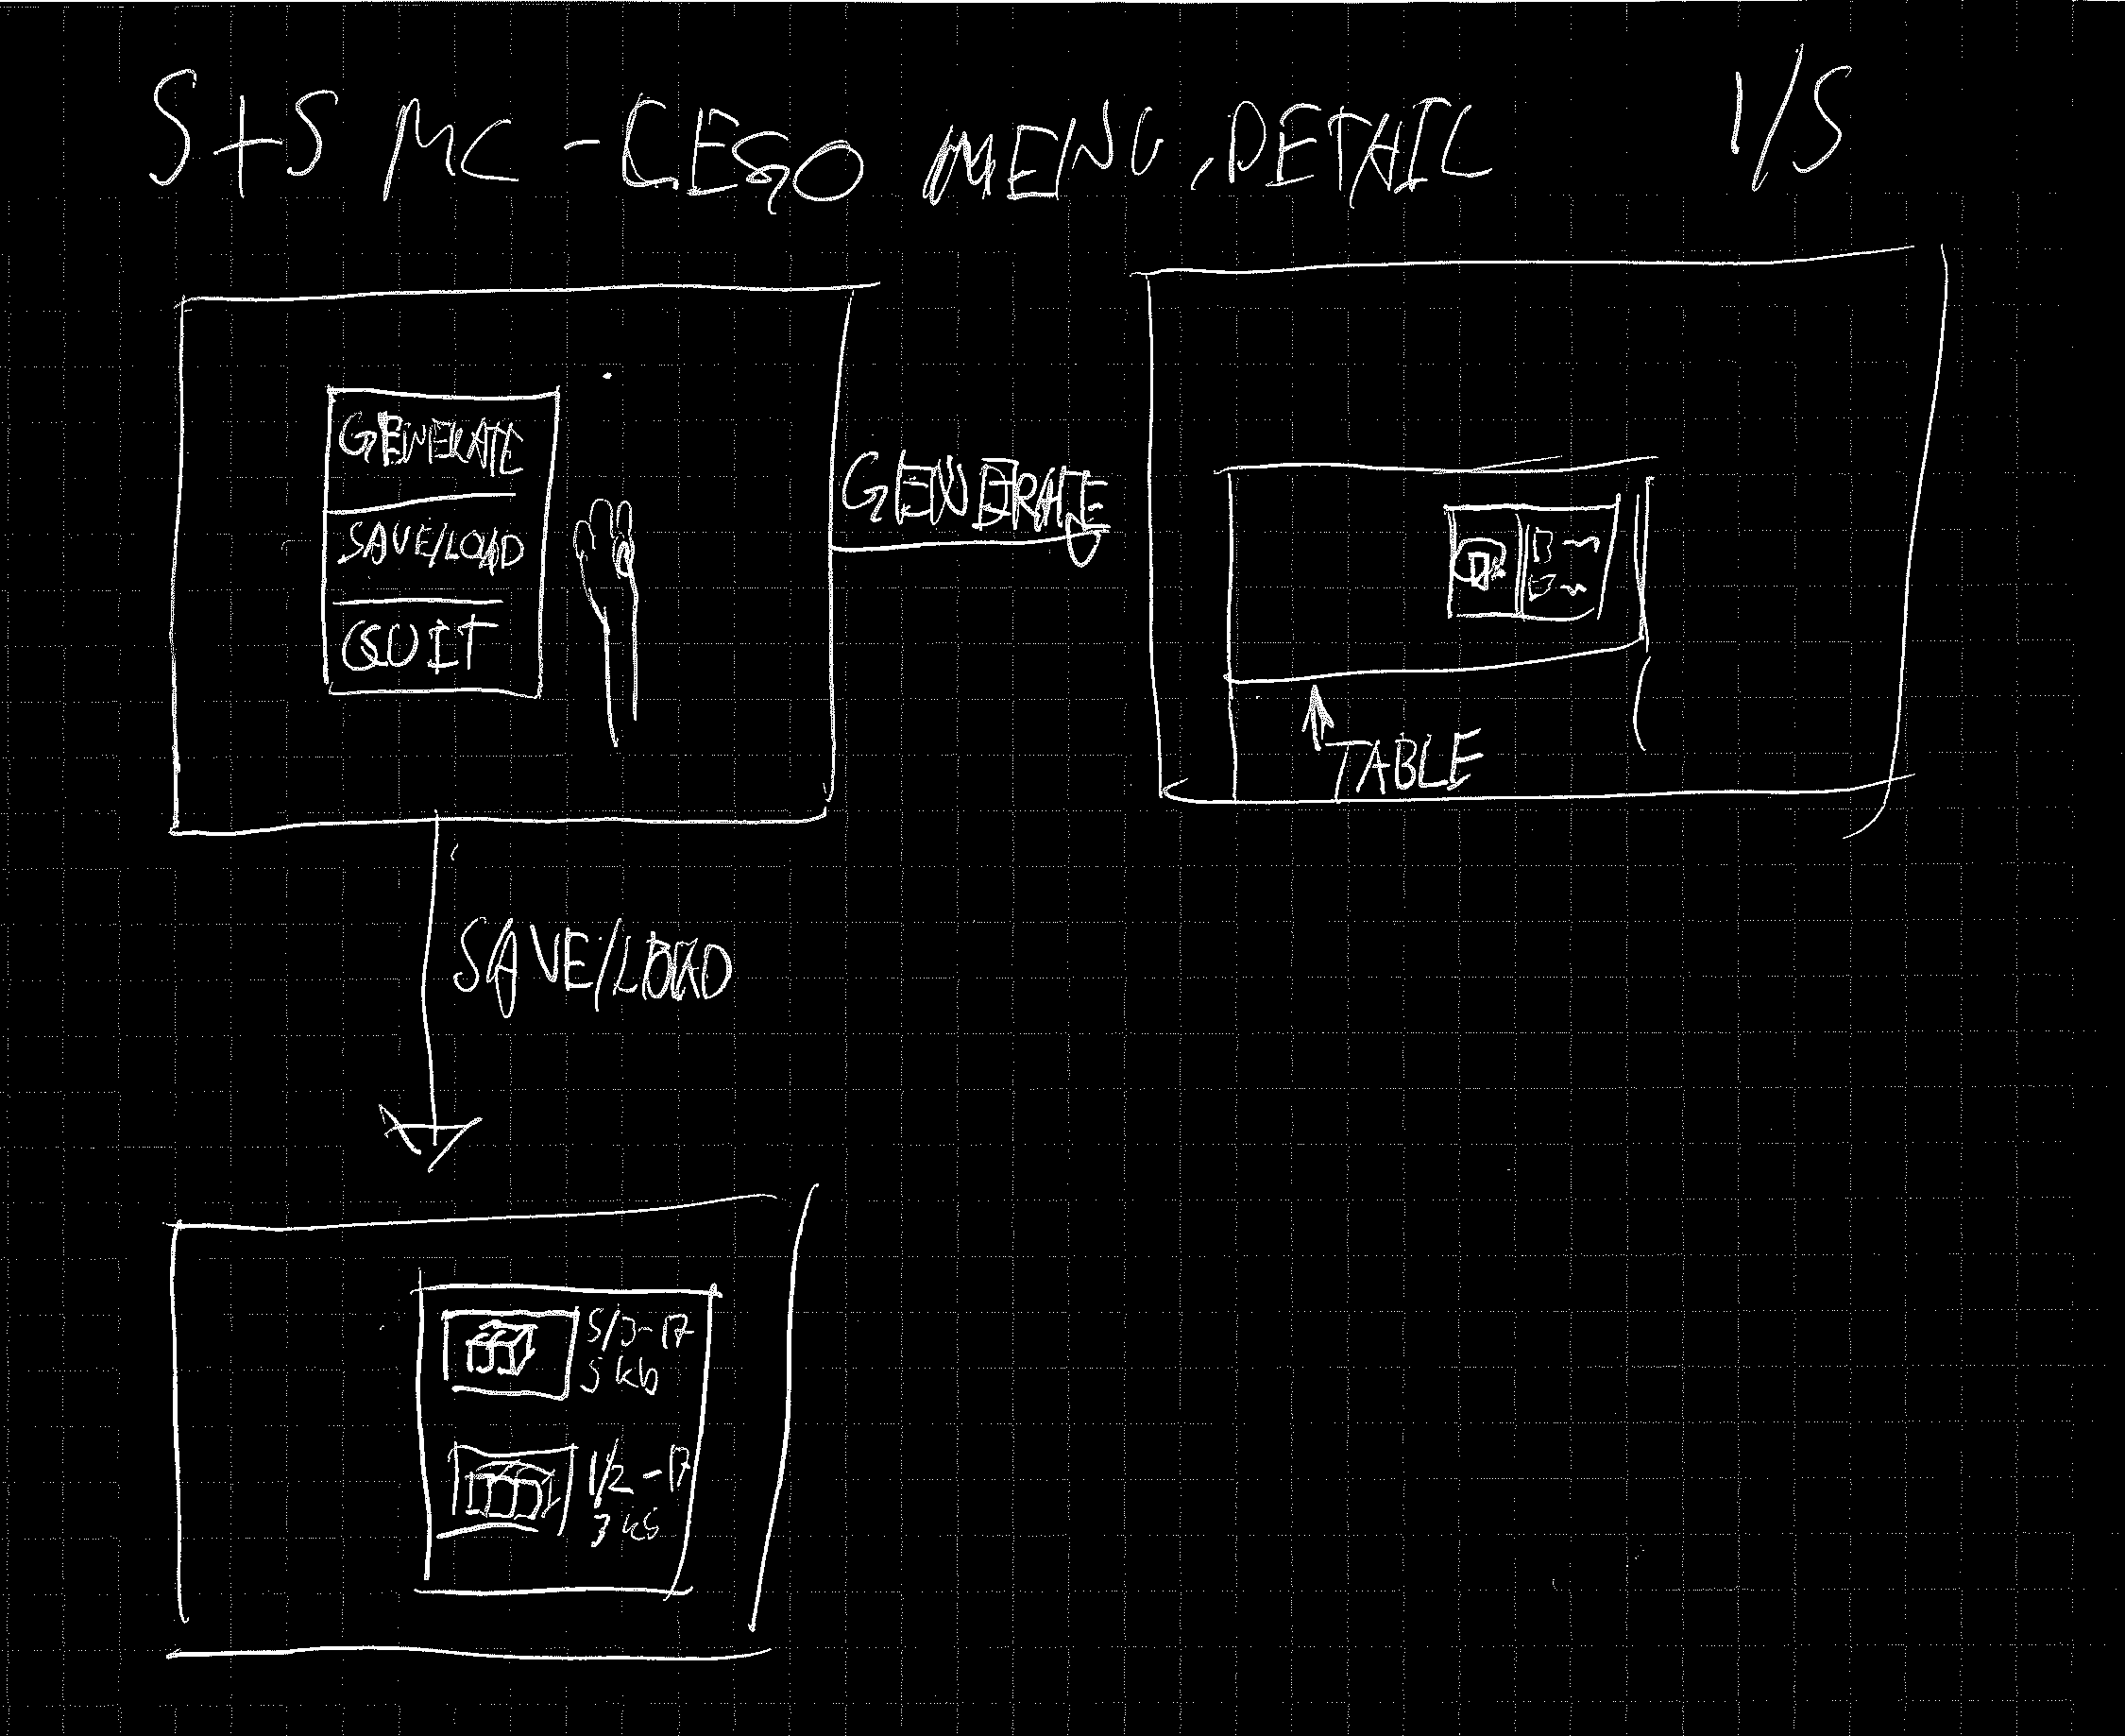
\includegraphics[width=0.7\linewidth]{figures/Menu/menu8}
	\caption{The first idea of a seperate Main Menu screen}
	\label{fig:menu8}
\end{figure}
The user would open the Hololens application, and be met with a menu screen, where actions such as generating a play area, loading and saving a game and a way to quit the application were possible. \par
One common theme in the sketching of the main menu was separating the design of the menu and the interaction techniques with the menu. This led to some sketches being focused on the interaction, such as figure \ref{fig:menugesture} depicts, and other sketches that solely focused on the menu design.\par
\begin{figure}[h]
	\centering
	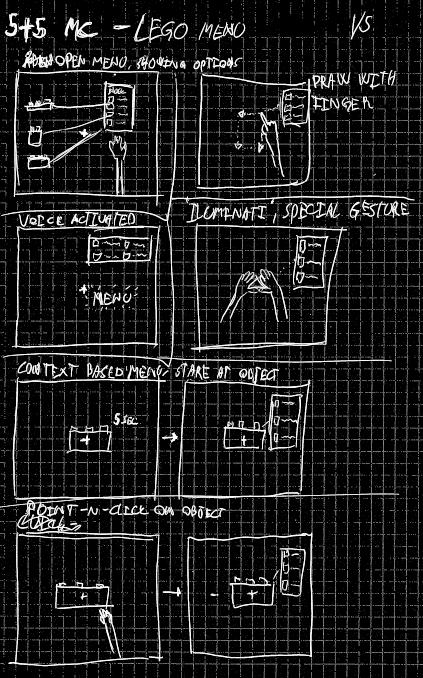
\includegraphics[width=0.7\linewidth]{figures/Menu/menu5}
	\caption{A focus on gestures rather than design, impacted the design. The figure shows 5 different ways of creating an interactive menu for the user to use.}
	\label{fig:menugesture}
\end{figure}
\par
The possibilities with the HoloLens gestures and the augmented reality made it apparent that the menu had to be movable, either by closing and opening with the gestures available, or being able to move it around the play area. 
\subsection{The Generator Board}
After discussing menus in the context of the Hololens, it became apparent that there was a need for a menu that could be placed and interacted within the real world. This menu should only interact inside the play area, and have functions tied to the bricks. Figure \ref{fig:genboard1} is a sketch of what functionalities the generator board could have.
\begin{figure}[h]
	\centering
	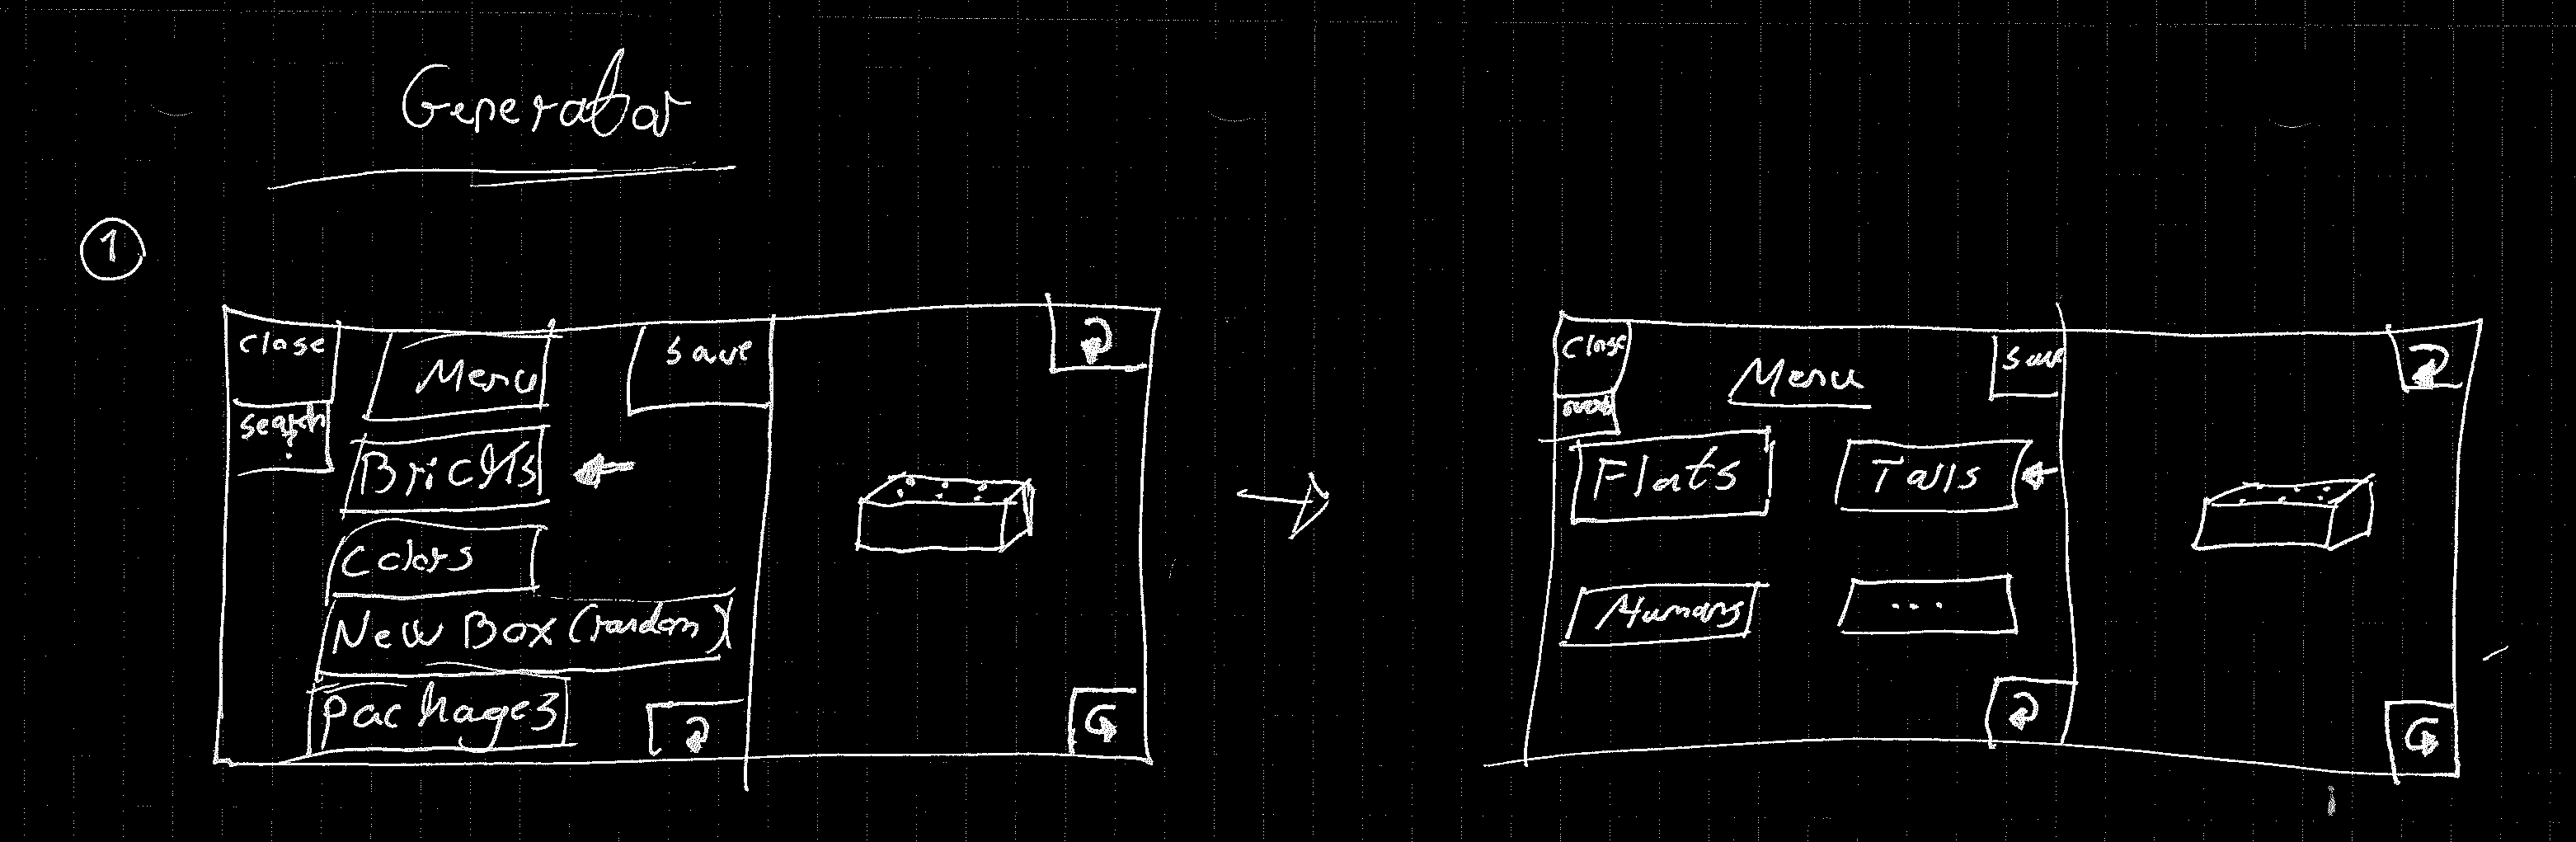
\includegraphics[width=0.7\columnwidth]{figures/Generator/gen5.png}
	\caption{An initial sketch of how the generator board could look like. The menu screen has alot of functionalities, and the actions chosen happen on the right side.}~\label{fig:genboard1}
\end{figure}
The generator board should be have functionalites that can alter the blocks, but also needs to be interactive and moveable in the play area.\par
Figure \ref{fig:gentablet} illustrates how the generator board is placed on a table and used for generating bricks.
\begin{figure}[h]
	\centering
	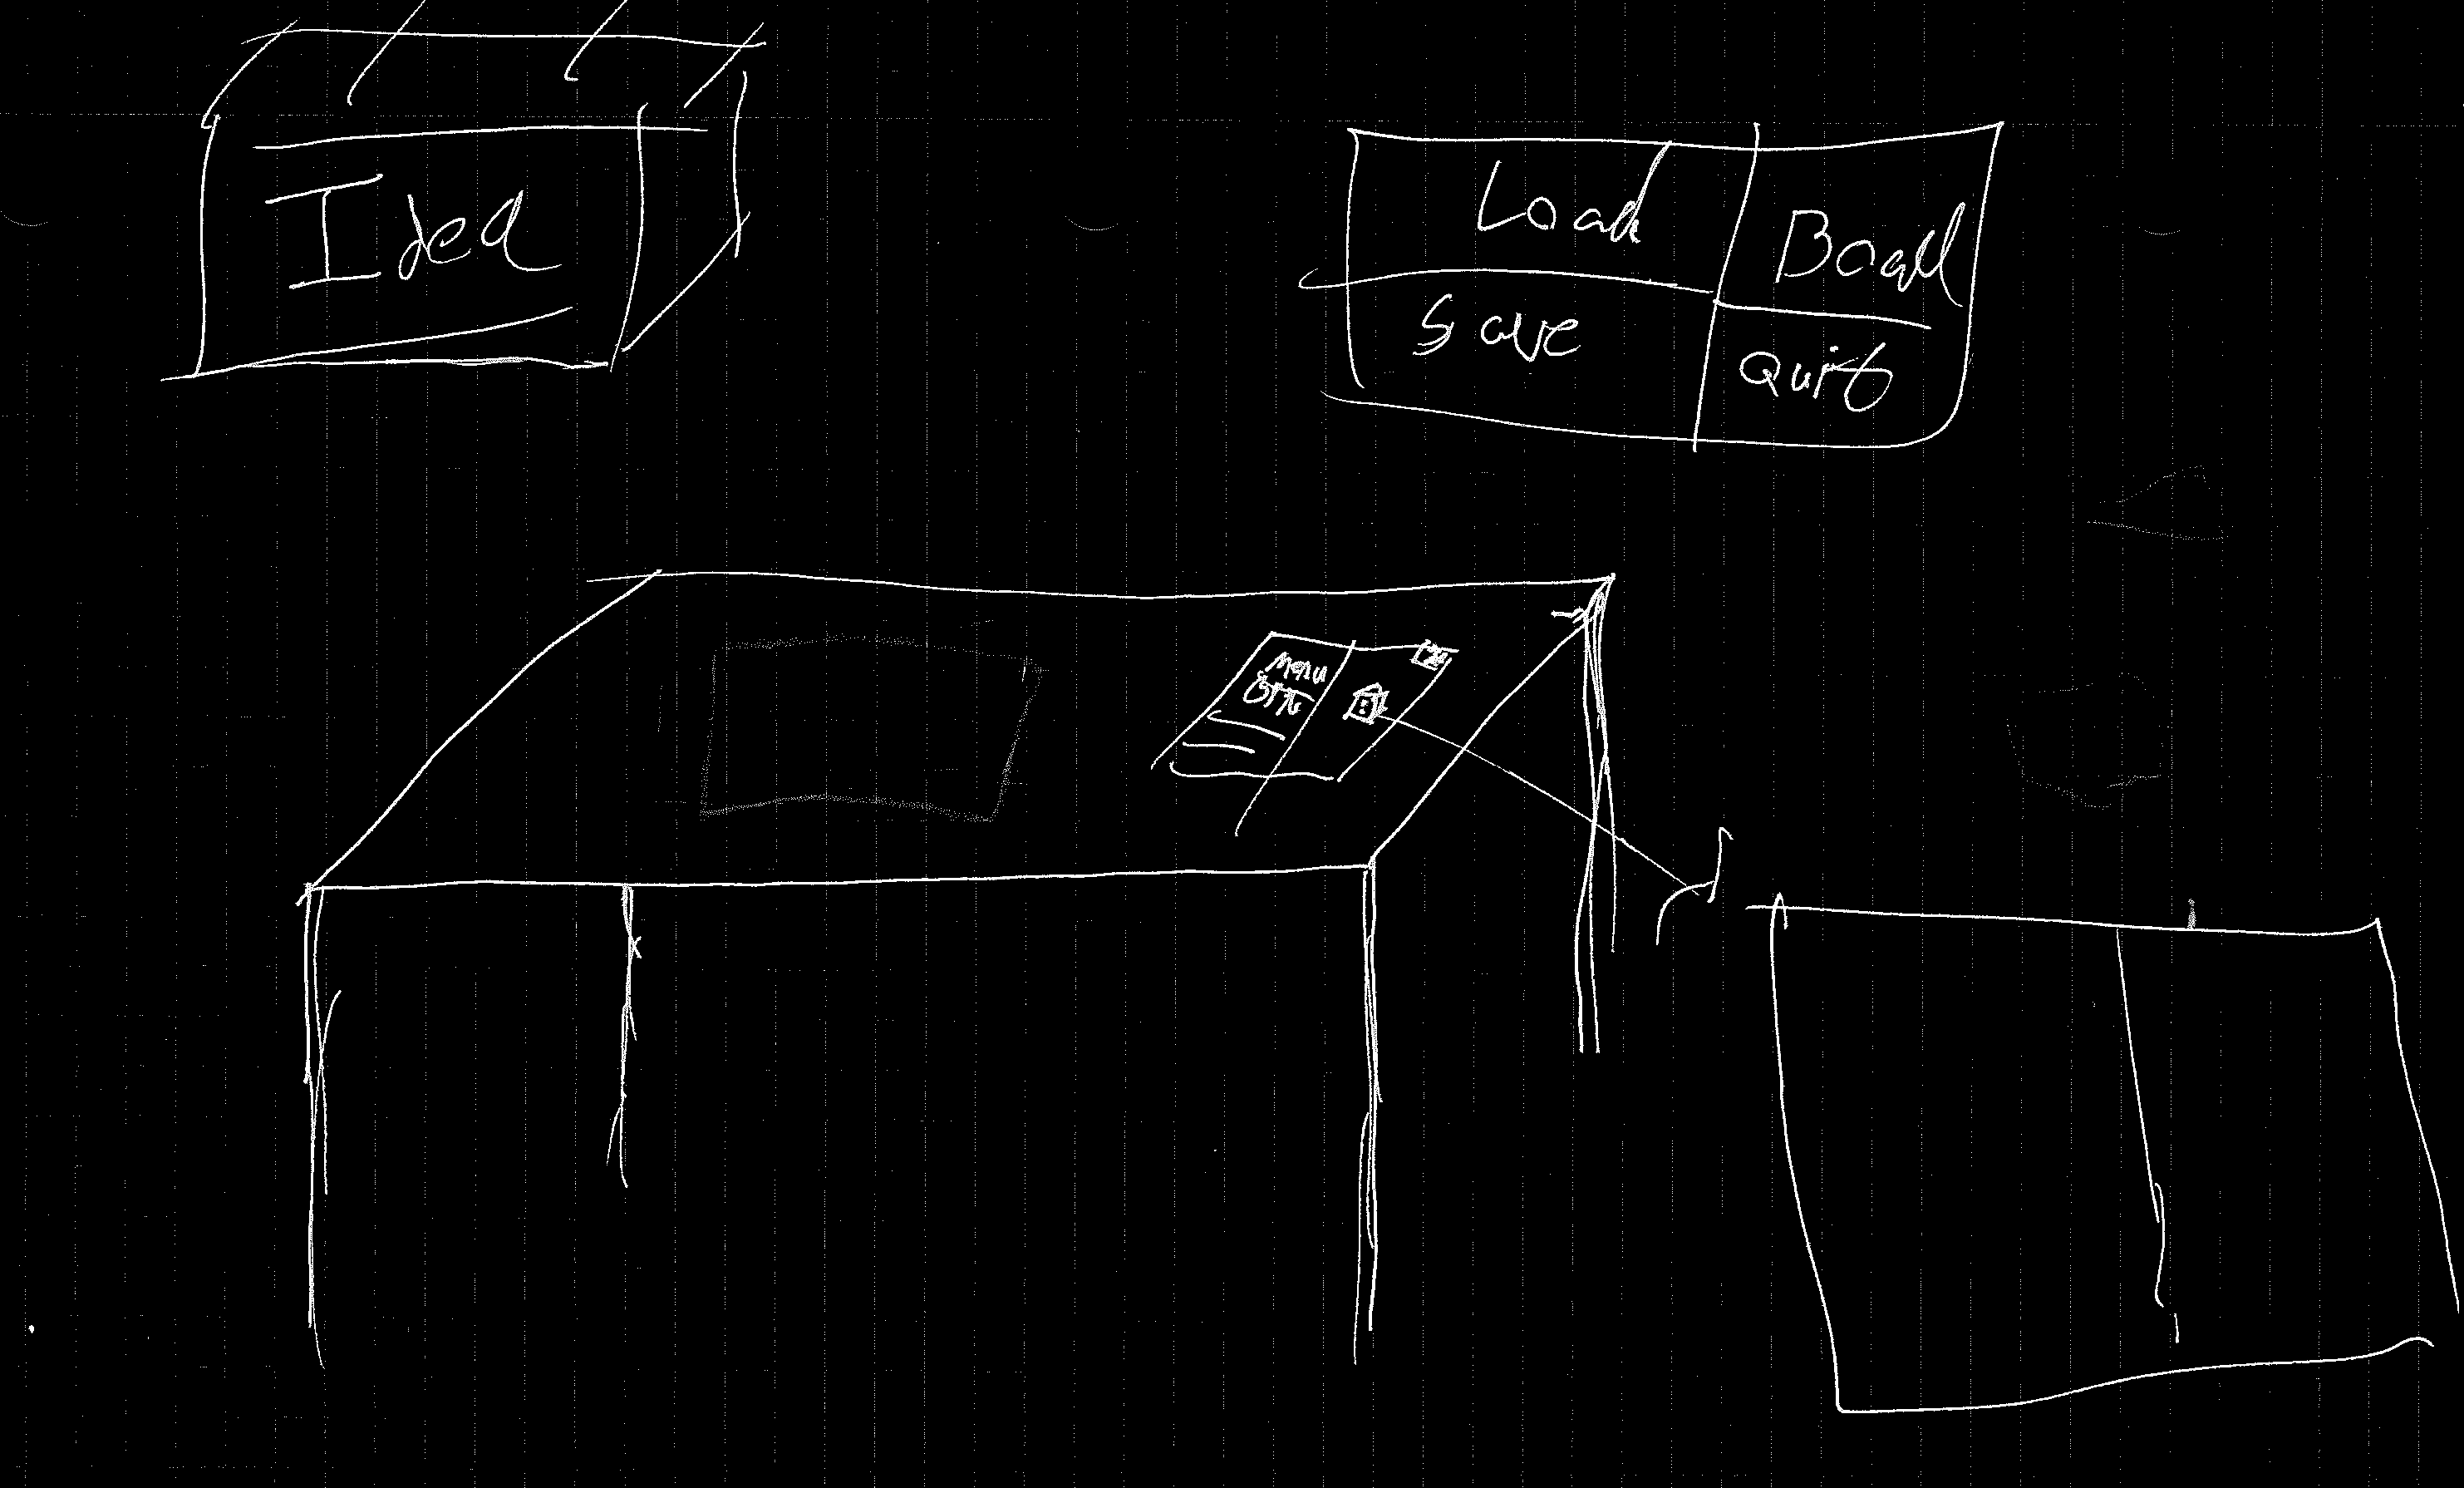
\includegraphics[width=0.7\columnwidth]{figures/Generator/gen6.png}
	\caption{First sketch of the generator board as a movable object. Here placed on the table, spawning blocks on the table.}~\label{fig:gentablet}
\end{figure}
We designed the generator board as a tablet device. Being a solid familar object, makes it more intuitive and natural for the user to interact with. To lift, move and place the tablet on a surface is a simple and familiar task for the user. To accompany the tablet device, a simple interface was designed. The interface only needed simple function all tied to spawning lego bricks. The user can spawn bricks of different types, change colors and saving/loading a play scene.
\subsection{Design Decisions}
\begin{figure}[h]
	\centering
	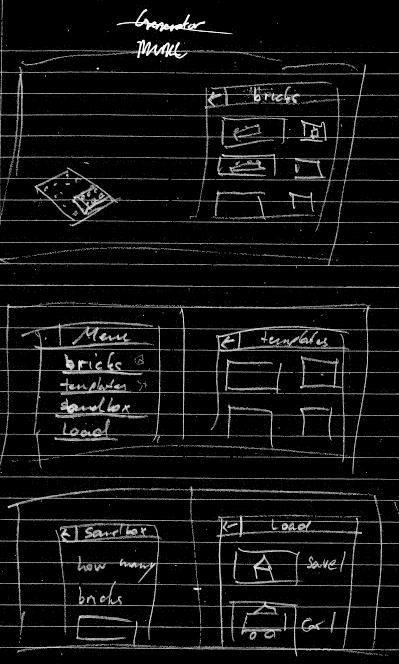
\includegraphics[width=0.5\columnwidth]{figures/Menu/menu1.png}
	\caption{Initial Main Menu screen with big buttons, simple interaction and short descriptions.}~\label{fig:genboard}
\end{figure}
During the sketching phase, several design choices were discussed. One of the very first concerns was the overall look of the main menu. The choice of big buttons, clear visual cues and short textual descriptions was present in almost all of the sketches in the early design phase, as seen in figure \ref{fig:genboard}. The generator board needed to have the same simple design. We decided The menus should not be overcomplicated, but not sparse in functions either.\par
As the development of the application progressed it became more  apparent that an actual main menu was not necessary. All the interactions needed for the prototype could be implemented  the tablet looking generator board and could ease user interaction with the application. Instead of going through a main menu and then having the generator which contains the functionality for working with the LEGO bricks, spawning the generator board at the application start up and "cutting out the middleman" seemed as a natural choice for this prototype. Granted, with an eventual increase in functionality and complexity of the application, a root/main menu might prove useful as to not clutter the users experience when they are building as opposed to when they are in the main menu setting options, loading scenarios, downloading templates etc. 



% !TeX root = ../proceedings.tex
\section{Implementation}

\subsection{Language and tools}
The LegoLens application is built using Unity, where custom scripts are written in C\#. Unity is chosen, since it is used in Microsofts own Hololens academy.\footnote{\url{https://developer.microsoft.com/en-us/windows/mixed-reality/academy}} Microsoft also provides a software toolkit called HoloToolkit\footnote{\url{https://github.com/Microsoft/HoloToolkit-Unity}}, which binds Unity and the Hololens together. \\
For initial testing the Microsoft Hololens Emulator was used, while in later stages the application was deployed directly to the Hololens device. 

\subsection{HoloToolkit}
The HoloToolkit provides implementations of common tasks in developing applications for the Hololens. This kit implements functionality which is mostly Hololens specific, such as spatial mapping and understanding. Also functionality for input methods are provided. The Hololens comes with two build-in gestures: the bloom and the tap.

\subsubsection{Spatial mapping and understanding}
These two functionalities are fundamental for the use of the Hololens, since they let the Hololens understand the shape of a room. Thereby virtual objects can be placed in the real world. The toolkit provides prefabricated functionality for mapping and understanding, which simply can be added in Unity.  \\
The Hololens uses a depth camera similar to the camera built into the Kinect v2 and four cameras meant to understand environment.\footnote{\url{https://developer.microsoft.com/en-us/windows/mixed-reality/hololens_hardware_details}} The spatial mapping relies on the time-of-flight Kinect-like depth camera and the four RGB cameras to provide a robust tracking of the enviroment. \\
This connection between the real-world and digital playground created in the application was essential, both to the experience but also to make the application augmenting the reality. The mapping allows to create a relative coordinate system, such that virtual objects can be placed in accurately.

\subsubsection{Input methods}
The Hololens tracks the gaze of the wearer, by the assumption that the wearer always looks straight ahead. This is the limitations of the Hololens, which does not provide augmentation for the whole field of view. Thus if the wearers eyes would be tracked, the wearer could gaze outside of the Hololens field of view. In this application a cursor appears where the gaze of the wearer collides with mapped objects in the real world or objects created by the application.\\ 
In this application the tap method is used. Here there are two different states the interaction can have: a single tap and dragging. \\
The single tap is used to navigate in the menu on the generator. The HoloToolkit provides functionality, such that objects can be dragged by holding tap. This is used to drag LEGO bricks and the generator around.

\subsection{Unity scripts}
While the HoloToolkit implements the augmentation of objects, the custom Unity scripts implement LEGO functionality. These scripts control the behaviour of the LEGO bricks, the generator and templates. 

\subsubsection{Generator}
The generator script contains the main functionality of the implemented code. Menu interactions are implemented here and thus the necessary functions to instantiate and model bricks. The instantiation is done by loading the prefabricated LEGO brick object, and colouring it depending on user input. A brick is not affected by gravity until the user interacts with the brick. For the purpose of initial simplicity the number of shapes a brick can have is limited. \\
Templates are implemented in a similar way as bricks, except that these can not be coloured. Also the sandbox feature is implemented in the generator script. It generates 20 bricks with random shape and colour. \\
The menu itself on the generator works by activating and deactivating the appropriate menu items.

\subsubsection{Bricks and Templates}
As described above, the brick and template scripts work in a similar way. They both make sure that the generated objects do not rotate and snap to a grid. A one-by-one brick is 0.8cm long and wide and 0.96cm tall (with knobs). Thus bricks are forced to be placed in positions which are multiples of 0.8.

% !TeX root = ../project.tex

\section{Discussion}

\subsection{Confusion and overwhelming impressions (H1)}
One aspect of the conducted tests was the apparent wow-factor of the HoloLens and virtual layer. The tests and observations showed that the subjects could not utilize the fact that the virtual layer extended beyond their apparent field-of-view. This resulted in many "out of sight, out of mind" situations, where the subjects tried to restart the application although nothing critical had happened. This can of course be explained and mediated using markers and other helping layers to indicate where the points of interest in the application may be located, but this would then in turn clutter an already sparse field-of-view. To ease the subjects into thinking in an AR setting we used the pre-existing "Learn Gestures" application, but this did not seem to have a strong beneficial impact on that issue.\\
The issue that H1 covers is under discussion in \cite{kim}. The results in \cite{kim} show that user studies need to be central in the development of AR as well as virtual reality applications. 

\subsection{Suitability of LEGO in AR (H2)}
One of the hypotheses introduced in the previous section was the suitability of LEGO in an AR setting. This question was asked rather late in the development process. What became apparent was that the virtual LEGO in an AR setting would not be able to provide the same "finicky" feel that LEGO does, sitting at a table, obsessing over small details in an advanced setup. This is because of the computational limitations of the HoloLens and the technology architecture. The minimal rendering distance of the HoloLens is, right now, much larger than the distance one would be from a real-life LEGO project, ie., arms length. This limitation demands a much larger brick size than real-life LEGO and this in turn limits the overall complexity of a virtual LEGO project. \\
These considerations became our main focus in the user tests: whether or not the HoloLens is applicable in these small scale, high detail applications such as LEGO. High detail, in this sense, refers to the many ways that LEGO bricks can be joined together to create more and more complex structures. With these structures comes problems, such as occlusions, tracking precision and stabilization issues. 

% !TeX root = ../proceedings.tex

\section{Future work}

\subsection{Hypothesis specific}
To work with these hypotheses, more tests would have to be conducted, but also the application stability would have to improve dramatically. Users have to feel confident in the application so as to reveal any problems with AR interaction methods as a whole, so that any frustrations and considerations are directed against AR instead of AR AND the application.\\
\\
With regards to H2, tests showed that brick size, ease of access through the menu and a general handholding of the user (in our case, bricks being locked in rotation and snapping to a virtual grid) improved the LEGO experience in an AR setting. Since the technology is not fully developed it is difficult to specify best parameters such as brick size and functionalities that would improve precision. The test subjects showed a general consensus in that LEGO was suitable for AR. One problem is that they only had one point of reference, our high fidelity, but unfinished prototype, and thus it becomes a very subjective matter whether the brick size is actually of an appropriate size or if LEGO as a whole makes sense in AR.\\
One way of narrowing down specific parameters would be a comparative approach to testing, ie. a prototype with different bricks sizes, functionalities and input methods. 

\subsection{Application specific}
To combat the issue with the size of actual LEGO and the complexity available in this scale a virtual magnifying glass could be envisioned. Using a special gesture, a certain area of the LEGO bricks could be brought into view using a secondary "screen", a menu that could show a zoomed in version of the actual view the user has, such as a magnifying glass.\\
\\
The number of input methods implemented into the HoloLens is limited and this is what a test subject criticized. Thus an extension of the input methods is an obvious next step to take. Here the choice of extensions ranges from implementing more hand gestures to using methods such as WatchSense \cite{watchsense}, which utilizes SmartWatches and gestures on the back of the hand to provide a new interaction method. \\
\\
There is a severe shortage of bricks available in the prototype. Anyone who considers an AR LEGO application will soon have to think of which set of blocks or types they would include. The amount of distinctive LEGO bricks is staggeringly high, and this sort of work would probably benefit greatly from working together with LEGO as to get dimensions and oddities right. This work would also make such an application much more attractive, as one of the strongest selling points of LEGO is the variety, but ensured compatibility.\\
\\
Improving the stability of the spatial mapping would have to be a top priority if the prototype is to evolve from the state that it is in at the moment. To many disappearing bricks and generators end up with confused users, which is very troublesome taking H1 into consideration. 

\begin{figure}
\centering
  %\includegraphics[width=0.9\columnwidth]{figures/sigchi-logo}
  \caption{Insert a caption below each figure. Do not alter the
    Caption style.  One-line captions should be centered; multi-line
    should be justified. }~\label{fig:figure1}
\end{figure}

\begin{table}
  \centering
  \begin{tabular}{l r r r}
    % \toprule
    & & \multicolumn{2}{c}{\small{\textbf{Test Conditions}}} \\
    \cmidrule(r){3-4}
    {\small\textit{Name}}
    & {\small \textit{First}}
      & {\small \textit{Second}}
    & {\small \textit{Final}} \\
    \midrule
    Marsden & 223.0 & 44 & 432,321 \\
    Nass & 22.2 & 16 & 234,333 \\
    Borriello & 22.9 & 11 & 93,123 \\
    Karat & 34.9 & 2200 & 103,322 \\
    % \bottomrule
  \end{tabular}
  \caption{Table captions should be placed below the table. We
    recommend table lines be 1 point, 25\% black. Minimize use of
    table grid lines.}~\label{tab:table1}
\end{table}

\begin{figure*}
  \centering
 % \includegraphics[width=1.75\columnwidth]{figures/map}
  \caption{In this image, the map maximizes use of space. You can make
    figures as wide as you need, up to a maximum of the full width of
    both columns. Note that \LaTeX\ tends to render large figures on a
    dedicated page. Image: \ccbynd~ayman on
    Flickr.}~\label{fig:figure2}
\end{figure*}
<<<<<<< HEAD
\nocite{*}
=======

\nocite{*}

>>>>>>> 5de5dcc71570b631c30f45f76a51a5783c2d956b
% REFERENCES FORMAT
% References must be the same font size as other body text.
\bibliographystyle{SIGCHI-Reference-Format}
\bibliography{sample.bib}

\end{document}

%%% Local Variables:
%%% mode: latex
%%% TeX-master: t
%%% End:
